%\input{Preambulum}

\begin{figure}[t!]
\centering

\begin{subfigure}{\textwidth}
\caption{Graphs with pair constraints ($G_1$--$G_{31}$ plus one pair of nodes, Figure~\ref{Fig1})}
\label{Fig6a}

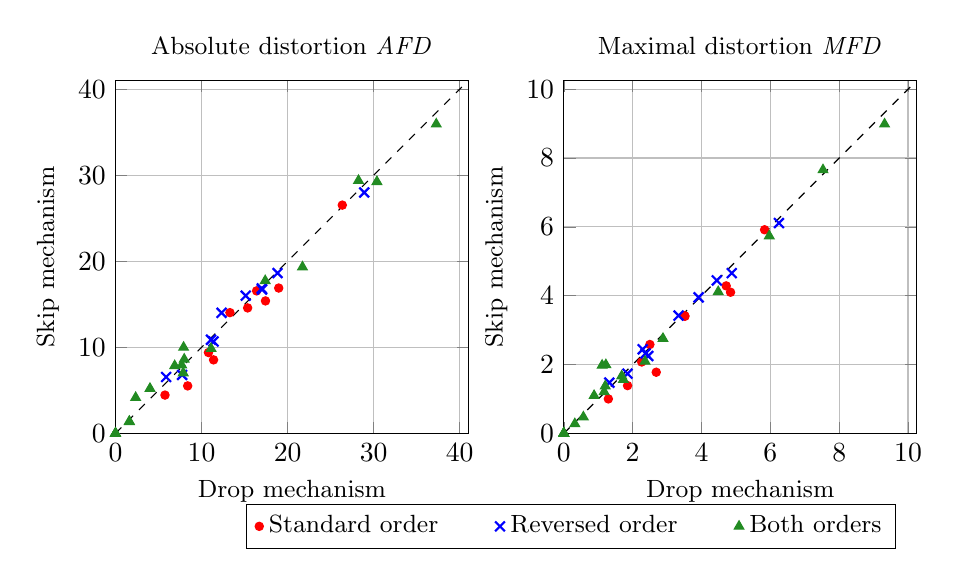
\begin{tikzpicture}
\begin{axis}[
name = axis1,
title = {Absolute distortion $\mathit{AFD}$},
title style = {font=\small},
xlabel = Drop mechanism,
x label style = {font=\small},
ylabel = Skip mechanism,
y label style = {font=\small},
width = 0.5\textwidth,
height = 0.5\textwidth,
nodes near coords,
xmajorgrids = true,
ymajorgrids = true,
xmin = 0,
xmax = 41,
ymin = 0,
ymax = 41,
]
\addplot [scatter,red,only marks,mark size=1.5pt,point meta=explicit symbolic] coordinates {
(5.75196408529747,4.45566778900112)
(8.38779956427025,5.52287581699346)
(13.2988380537401,14.0359477124183)
(10.8035371011149,9.39830834294502)
(17.4300044091711,15.3968253968254)
(18.9670138888888,16.8923611111111)
(16.3966049382716,16.5625)
(26.3558201058201,26.5277777777778)
(11.3960113960113,8.54700854700854)
(15.3549382716051,14.5833333333333)
};
\addplot [scatter,blue,only marks,mark=x,mark size=2.5pt,thick,point meta=explicit symbolic] coordinates {
(5.88056490834269,6.55443322109989)
(7.74328249818459,6.79738562091503)
(12.3275236020334,14.0114379084967)
(11.0985625186893,10.8852364475202)
(17.0345568783069,16.7162698412698)
(16.9959766313932,16.8576388888889)
(15.1331018518517,16.0069444444444)
(28.9021164021163,27.9960317460317)
(11.3960113960115,10.6837606837607)
(18.827160493827,18.6342592592592)
};
\addplot [scatter,ForestGreen,only marks,mark=triangle*,mark size=2pt,point meta=explicit symbolic] coordinates {
(0,0)
(2.34250398724091,4.16267942583732)
(0,0)
(4.00891632373112,5.21604938271604)
(7.91340218423561,9.99287749287749)
(7.87037037037033,7.02614379084968)
(11.1082444673777,9.85552115583075)
(7.69562454611469,7.93300653594771)
(0,0)
(0,0)
(1.60108024691384,1.3888888888889)
(21.728570426487,19.3292297979798)
(28.2366071428573,29.3799603174603)
(30.3780864197532,29.25)
(37.2727272727272,35.9393939393939)
(7.98611111111113,8.61111111111111)
(17.3960170487948,17.7380952380953)
(6.878306878307,7.85714285714285)
(0,0)
(1.62337662337664,1.35281385281388)
(0,0)
};
% Zero line
\draw [black,dashed] (rel axis cs:0,0) -- (rel axis cs:1,1);
\end{axis}

\begin{axis}[
at = {(axis1.south east)},
xshift = 0.1\textwidth,
title = {Maximal distortion $\mathit{MFD}$},
title style = {font=\small},
xlabel = Drop mechanism,
x label style = {font=\small},
ylabel = Skip mechanism,
y label style = {font=\small},
width = 0.5\textwidth,
height = 0.5\textwidth,
nodes near coords,
xmajorgrids = true,
ymajorgrids = true,
xmin = 0,
xmax = 10.25,
ymin = 0,
ymax = 10.25,
legend style = {font=\small,at={(-0.9,-0.2)},anchor=north west,legend columns=3},
legend entries = {Standard order$\qquad$,Reversed order$\qquad$,Both orders}
]
\addplot [scatter,red,only marks,mark size=1.5pt,point meta=explicit symbolic] coordinates {
(1.2941919191919,1.00252525252525)
(2.68518518518526,1.77777777777778)
(3.51273148148151,3.41666666666667)
(2.26307189542483,2.07516339869281)
(4.84347442680776,4.10119047619048)
(4.71781305114639,4.28571428571429)
(2.50000000000009,2.58333333333334)
(5.83333333333331,5.91666666666667)
(1.85185185185186,1.38888888888889)
(3.5185185185185,3.40277777777778)
};
\addplot [scatter,blue,only marks,mark=x,mark size=2.5pt,thick,point meta=explicit symbolic] coordinates {
(1.32312710437707,1.47474747474748)
(2.45370370370376,2.25)
(3.33333333333335,3.42361111111111)
(2.37495461147419,2.32516339869281)
(4.87819664903005,4.65674603174603)
(3.91644620811283,3.95238095238095)
(2.29166666666673,2.44444444444444)
(6.24999999999996,6.11111111111111)
(1.85185185185188,1.73611111111111)
(4.44444444444441,4.44444444444444)
};
\addplot [scatter,ForestGreen,only marks,mark=triangle*,mark size=2pt,point meta=explicit symbolic] coordinates {
(0,0)
(1.11268939393942,1.97727272727273)
(0,0)
(1.17206790123456,1.20833333333333)
(1.22188093542263,1.99252136752137)
(1.6820987654321,1.66666666666667)
(2.36050194931776,2.09429824561403)
(1.73032407407407,1.5625)
(0,0)
(0,0)
(0.320216049382771,0.277777777777777)
(4.48565516273854,4.11489898989899)
(7.52976190476193,7.65476190476191)
(5.96836419753091,5.73611111111111)
(9.31818181818183,8.98484848484848)
(0.879629629629657,1.09722222222223)
(2.88111772486773,2.75496031746032)
(1.2037037037037,1.375)
(0,0)
(0.568181818181798,0.473484848484848)
(0,0)
};
% Zero line
\draw [black,dashed] (rel axis cs:0,0) -- (rel axis cs:1,1);
\end{axis}
\end{tikzpicture}
\end{subfigure}

\vspace{0.25cm}
\begin{subfigure}{\textwidth}
\caption{Graphs without pair constraints ($H_1$--$H_{31}$ plus one pair of nodes, Figure~\ref{Fig2})}
\label{Fig6b}

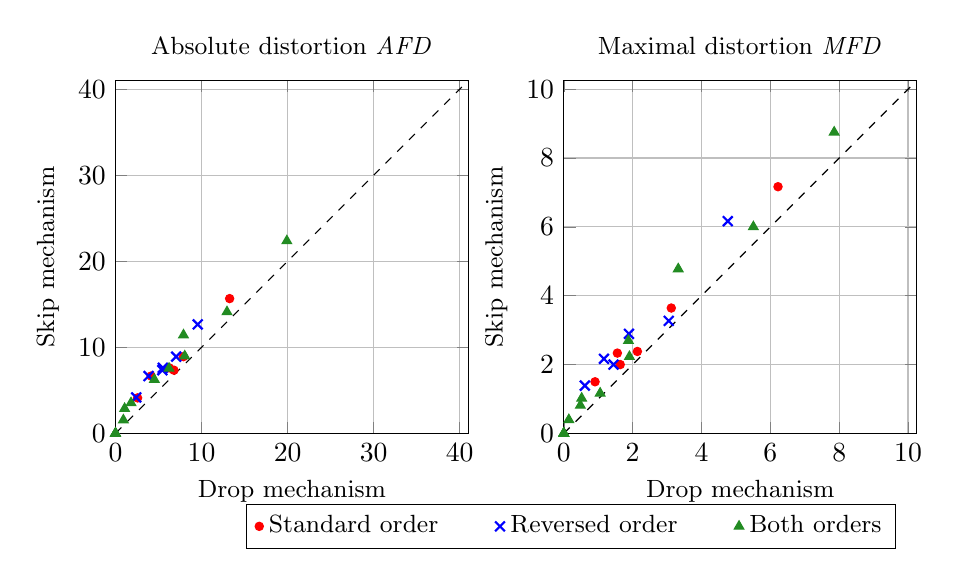
\begin{tikzpicture}
\begin{axis}[
name = axis1,
title = {Absolute distortion $\mathit{AFD}$},
title style = {font=\small},
xlabel = Drop mechanism,
x label style = {font=\small},
ylabel = Skip mechanism,
y label style = {font=\small},
width = 0.5\textwidth,
height = 0.5\textwidth,
nodes near coords,
xmajorgrids = true,
ymajorgrids = true,
xmin = 0,
xmax = 41,
ymin = 0,
ymax = 41,
]
\addplot [scatter,red,only marks,mark size=1.5pt,point meta=explicit symbolic] coordinates {
(4.14141414141424,6.66666666666666)
(2.56613756613751,4.12698412698412)
(6.24338624338617,7.61904761904762)
(7.89566508864749,8.92230576441104)
(6.79138321995467,7.34693877551021)
(13.2638888888888,15.6666666666667)
};
\addplot [scatter,blue,only marks,mark=x,mark size=2.5pt,thick,point meta=explicit symbolic] coordinates {
(3.83838383838391,6.66666666666666)
(2.40740740740732,4.17989417989418)
(5.50264550264545,7.61904761904762)
(7.05096073517122,8.92230576441103)
(5.44217687074826,7.34693877551021)
(9.55555555555559,12.6666666666667)
};
\addplot [scatter,ForestGreen,only marks,mark=triangle*,mark size=2pt,point meta=explicit symbolic] coordinates {
(0,0)
(0,0)
(1.80602006688967,3.54515050167223)
(1.06060606060613,2.87878787878788)
(0.916442048517484,1.55136268343816)
(0,0)
(7.90123456790121,11.4285714285714)
(4.51929012345677,6.25)
(0,0)
(6.22222222222225,7.55555555555556)
(8.0495219530306,8.98078529657478)
(12.9557007988381,14.1176470588235)
(0,0)
(19.9122807017544,22.3684210526316)
};
% Zero line
\draw [black,dashed] (rel axis cs:0,0) -- (rel axis cs:1,1);
\end{axis}

\begin{axis}[
at = {(axis1.south east)},
xshift = 0.1\textwidth,
title = {Maximal distortion $\mathit{MFD}$},
title style = {font=\small},
xlabel = Drop mechanism,
x label style = {font=\small},
ylabel = Skip mechanism,
y label style = {font=\small},
width = 0.5\textwidth,
height = 0.5\textwidth,
nodes near coords,
xmajorgrids = true,
ymajorgrids = true,
xmin = 0,
xmax = 10.25,
ymin = 0,
ymax = 10.25,
legend style = {font=\small,at={(-0.9,-0.2)},anchor=north west,legend columns=3},
legend entries = {Standard order$\qquad$,Reversed order$\qquad$,Both orders}
]
\addplot [scatter,red,only marks,mark size=1.5pt,point meta=explicit symbolic] coordinates {
(1.5555555555556,2.33333333333334)
(0.907407407407429,1.5)
(1.63888888888892,2)
(2.13712522045853,2.38095238095238)
(3.12202380952388,3.64285714285715)
(6.22222222222223,7.16666666666667)
};
\addplot [scatter,blue,only marks,mark=x,mark size=2.5pt,thick,point meta=explicit symbolic] coordinates {
(1.16666666666665,2.16666666666667)
(0.61111111111109,1.38888888888888)
(1.44444444444448,2)
(3.04761904761908,3.26984126984127)
(1.89285714285721,2.89285714285715)
(4.7638888888889,6.16666666666667)
};
\addplot [scatter,ForestGreen,only marks,mark=triangle*,mark size=2pt,point meta=explicit symbolic] coordinates {
(0,0)
(0,0)
(0.51923076923075,1.01923076923077)
(0.145833333333362,0.395833333333334)
(0.48113207547171,0.814465408805032)
(0,0)
(3.32407407407409,4.77777777777778)
(1.87731481481482,2.69444444444444)
(0,0)
(1.05555555555555,1.16666666666667)
(1.90608465608467,2.23015873015873)
(5.50617283950621,6)
(0,0)
(7.85416666666667,8.75)
};
% Zero line
\draw [black,dashed] (rel axis cs:0,0) -- (rel axis cs:1,1);
\end{axis}
\end{tikzpicture}
\end{subfigure}

\caption{Fairness distortions of the Drop and Skip mechanisms \\ for selected balanced bipartite graphs with 10 nodes}
\label{Fig6}
\end{figure}

%\end{document}